\documentclass{beamer}
\usepackage[utf8]{inputenc}
\usepackage{graphicx} %package to manage images
% \graphicspath{ {./images/chapter8} }
\usepackage{amsmath}
\usetheme{Berlin}
%\usecolortheme{beaver}
% Information to be included in the title page:
\title{Microwave Bipolar Transistors}
\subtitle{Chapter 9}
\author{Bonface~K.~M. \and Kanyi~Naftary}
\institute{
  Department of Electrical and Electronic Engineering \\
  University of Nairobi
}
\date{October 2017}

\begin{document}

\frame{\titlepage}
\begin{frame}
  \frametitle{Table of Contents}
  \tableofcontents
\end{frame}

%%%%%%%%%%%%%%%%
% Introduction %
%%%%%%%%%%%%%%%%
\section{Introduction}
\begin{frame}
  \frametitle{Introduction}
  A Microwave Bipolar Transistors is a non-linear devices. Its principle of operation is similar to that of low frequency BJTs. \emph{Higher interelectrode capacitance, lead inductance} and \emph{transit time} limit the low frequency BJTs at \textbf{high frequencies}. Thus \emph{proper geometry} to reduce the above effects, \emph{process control, heat sinking and packaging} are first and foremost criteria for the designing of a high frequency transistor.

  All Microwave Bipolar Transistors are planar in form and of the n-p-n type. As mobility of electron($\mu_e$) is greater than that of hole($\mu_h$), hence electron emitted by the emitter of an n-p-n transistor will reach collector faster than the hole and which in turn the speed of operation.

  Moder Microwave Bipolar Transistors can operate at frequencies of upto 22 Ghz
\end{frame}


%%%%%%%%%%%%%%%%%%%%%%
% Physical Structure %
%%%%%%%%%%%%%%%%%%%%%%
\section{Physical Structure}
\begin{frame}
  \frametitle{Physical Structure}

  The geometry of Microwave Bipolar Transistors are important because they operate in high frequencies. The \emph{inter digitated geometry} consists of a large number of emitter strips alternating with base strips. The \emph{overlay geometry} has a large number of segmented emitters overlaid through a number of wide metal strips. The \emph{matrix/ mesh geometry}has an emitter that forms the grid, the base filling the meshes of this grid with a $p^+$ contact area in the middle of each mesh.
  Inter-digitated structure is suitable for small signal applications in the L, S and C bands whereas overlay and matrix structures are useful as power devices in VHF and UHF regions.
\end{frame}

\begin{frame}
  \begin{figure}[h]
    \caption{Geometrical Structures of microwave power transitor}
    \centering
    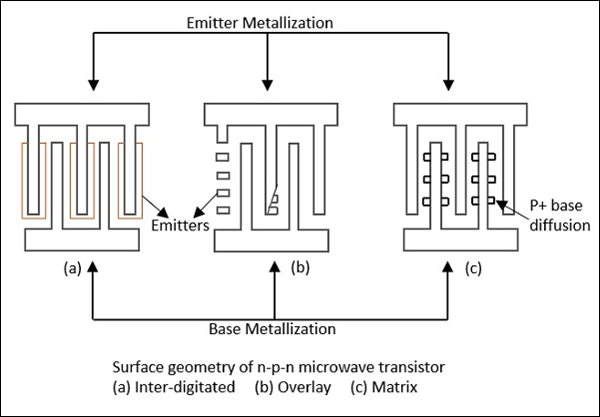
\includegraphics[width=0.4\textwidth]{./images/chapter9/fig9_1.png}
  \end{figure}
\end{frame}

%%%%%%%%%%%%%%%%%%%%%%%%%%
% Principle of Operation %
%%%%%%%%%%%%%%%%%%%%%%%%%%
\section{Principle Of Operation}
\begin{frame}
  \frametitle{Principle of Operation}
  A BJT can operate in 4 different modes:
  \begin{itemize}
  \item \textbf{Normal Mode}: Emitter junction of n-p-n transistoris forward biased and collector is reverse biased. Generally, at ON state a transistor remains in the normal mode.
  \item \textbf{Saturation Mode}: Both junctions are forward biased. Transistor acts like a short circuit.
  \item \textbf{Cut-off Mode}: Both junctions are reverse biased and transistor acts like an open circuit.
  \item \textbf{Inverse Mode}: Emitter is reverse biased and collector is forward biased. In practice, transistors are not commonly used in this mode.
  \end{itemize}
\end{frame}

\begin{frame}
    The microwave signal makes the base emitter junction forward biased at the negative portion of the signal and as a result electrons from the emitter region diffuses into the base and reaches the collector by drift mechanism. In the other half of the input signal the transistor remains in the OFF state, thus a pulse of current flows through the load connected in the collector circuit.
\end{frame}

%%%%%%%%%%%%%%%%%%%%%%%%%
% Performance Parameter %
%%%%%%%%%%%%%%%%%%%%%%%%%
\section{Performance Parameter}
\begin{frame}
  \frametitle{Performance Parameter}
  In high frequency operation of the performance of a microwave transistor depends on the cut off frequency,$f_c$, and maximum frequency of oscillation, $f_{max}$ rather than the 2 current gains $\alpha$ and $\beta$.

  \begin{align*}
    f_c &= \frac{1}{2\pi\tau_{ec}}\text{ ,where: } \\
    \tau_{ec} &= \tau_e + \tau_b + \tau_d + \tau_c\text{, and}\\
    \tau_e &= \text{Base Transit Time,}\\
    \tau_b &= \text{Base transit time,}\\
    \tau_d &= \text{Collector depletion layer transit time,}\\
    \tau_c &= \text{Collecter depletion layer charging time}
  \end{align*}
\end{frame}

\begin{frame}
  \begin{align*}
    f_{max} &= \sqrt{\frac{f_c}{8\pi r\sp{\prime}_{b}C_c}}, \\
    \text{where}\\
    r\sp{\prime}_{b} &= \text{Base resistance,}\\
    C_c &= \text{Collector capacitance}
  \end{align*}
\end{frame}

%%%%%%%%%%%%%%%%%%%%%%%%%%%%%%%
% Power Frequency Limitations %
%%%%%%%%%%%%%%%%%%%%%%%%%%%%%%%
\section{Power Frequency Limitations}
\begin{frame}
  \frametitle{Power Frequency Limitations}
  As the frequency is increased the output power drops mainly due to low impedance of the junction capacitance. The power frequency limitation is due to the:
  \begin{itemize}
  \item maximum velocity of charge carriers in a semiconductor($6 \times 10^6$cm/s in Ge of Si).
  \item the maximum electric field that can be applied to a semiconductor is $2 \times 10^5$V/cm
  \item the base width determines the maximum current
  \end{itemize}
\end{frame}

\begin{frame}
  \begin{columns}

    \column{0.5\textwidth}
    Let $V_m$ be the maximum applied voltage and the corresponding current be $I_m$ and if the charge carrier takes $\tau_{ec}$ time to cross the length L of the device, then:
    \column{0.5\textwidth}
    \begin{align*}
      V_m . f_c &= \frac{V_m}{L}. \frac{L}{2\pi\tau_ec}\\
                &= \frac{E_mV_s}{2\pi}\\
      \text{where }
      E_m &= \text{Maximum electric field}\\
                &= \frac{V_m}{L}\\
      \text{and }
    \end{align*}
    \begin{align*}
      v_s &= \text{Saturated drift velocity of the carrier}\\
            &= \frac{L}{\tau_{ec}}
    \end{align*}
  \end{columns}
\end{frame}

\begin{frame}
  \begin{columns}
    \column{0.5\textwidth}
    \begin{align*}
      X_c &= \frac{1}{\omega_{c}C_{bc}} = \frac{1}{2\pi f_{c}C_{bc}}\\
      \Rightarrow (I_mX_c).f_c &= \frac{E_mv_s}{2\pi}
    \end{align*}
    The max power dissipated across $X_c$ is:
    \begin{align*}
      P_m &= I_m^2X_c\\
      \Rightarrow I_m = \sqrt{\frac{P_m}{X_c}}\\
      \therefore (P_mX_c)^{\frac{1}{2}}f_c &= \frac{E_mv_s}{2\pi}
    \end{align*}
    $f_c = \frac{E_mv_s}{2\pi}.\frac{1}{\sqrt{X_xP_m}}  \Rightarrow f_c \propto \frac{1}{\sqrt{P_m}} $
    \column{0.5\textwidth}
    The gain frequency relation is given by:
    $$(G_m.V_{th}V_{m})^{\frac{1}{2}}.f = \frac{E_mV_s}{2\pi}$$
    where:
    \begin{align*}
      G_m &= \text{maximum available power gain}\\
      V_{th} &= \frac{kT}{e} \text{ is the thermal voltage}\\
      k &= \text{Boltzmann constant}\\
      f &= \text{Frequency of operation}
    \end{align*}
  \end{columns}
\end{frame}

\begin{frame}
  The input capacitance($C_{in}$)and the emitter diffusion capacitance $C_d$ are related by:
  $$C_{in} \approx C_d \cong \frac{Q_{m}}{V_{th}} \cong \frac{I_m.\tau_b}{V_{th}}$$
  The output capacitance is given by:
  $$C_{out} = C_{bc} = \frac{I_m.\tau_{ec}}{V_m}$$
\end{frame}

%%%%%%%%%%%%%%%%
% Applications %
%%%%%%%%%%%%%%%%
\section{Applications}
\begin{frame}
  \frametitle{Applications}
  Microwave Bipolar Transistor is used in \emph{L-band} transmitters for telemetry systems and phased array radar systems.

  It is also used in L and S band transmitters for communication systems.
\end{frame}

%%%%%%%%%%%%%%%%%%%%%%%%%%%%%%%%%%%%
% Heterogenous Bipolar Transistors %
%%%%%%%%%%%%%%%%%%%%%%%%%%%%%%%%%%%%
\section{Heterogenous Bipolar Transistors}
\begin{frame}
  \frametitle{Heterogenous Bipolar Transistors}
  \framesubtitle{Definition}
  Transistor junctions formed by 2 similar materials(such as silicon) is known as homojunction transistor, whereas the transistor junction formed by 2 different materials such as Ge to GaAs is called \emph{heterojunction transistor.}
\end{frame}

%%%%%%%%%%%%%%%%%%%%%
% Structure of HBTs %
%%%%%%%%%%%%%%%%%%%%%
\section{Structure of HBTs}
\begin{frame}
  \frametitle{Heterogenous Bipolar Transistors}
  \framesubtitle{Structure and Application of heterogenous transistors}
  Two materials can be used to fabricate a heterojunction transistor when their lattice constants are matched. Otherwise mismatch of lattice constants introduce a large number of inteface states and degrades the heterojunction operation.

  HBTs are mainly used for high speed switching devices in the microwave frequencies.
\end{frame}

%%%%%%%%%%%%%%%%%%%%%%%%
% Applications of HBTs %
%%%%%%%%%%%%%%%%%%%%%%%%
%\section{Applications of HBTs}
%\input{./hbtApplications.tex}

\end{document}